%% -*- coding: utf-8 -*-
\documentclass[12pt,a4paper]{scrartcl} 
\usepackage[utf8]{inputenc}
\usepackage[english,russian]{babel}
\usepackage{indentfirst}
\usepackage{misccorr}
\usepackage{graphicx}
\usepackage{amsmath}
\usepackage{float}
\usepackage{ dsfont }

\usepackage{xcolor}
\usepackage{hyperref}
\hypersetup{colorlinks,
  pdftitle={The title of your document},
  pdfauthor={Your name},
  allcolors=[RGB]{000 000 000}}

\begin{document}
\begin{titlepage}
  \begin{center}

    Санкт-Петербургский политехнический университет Петра Великого

    \vspace{0.25cm}
    
    Институт прикладной математики и механики
    
    Кафедра «Прикладная математика»
    \vfill

	\vspace{0.25cm}
	    Отчёт\\
	по лабораторной работе №5\\
	по дисциплине\\
	«Вычислительные комплексы»

  \bigskip

\end{center}
\vfill

\newlength{\ML}
\settowidth{\ML}{«\underline{\hspace{0.7cm}}» \underline{\hspace{2cm}}}
\hfill\begin{minipage}{0.4\textwidth}
  Выполнил студент\\ В.\,А.~Рыженко\\
\end{minipage}%
\bigskip

\hfill\begin{minipage}{0.4\textwidth}
  Проверил:\\
к.ф.-м.н., доцент\\
Баженов Александр Николаевич\\
\end{minipage}%
\vfill

\begin{center}
  Санкт-Петербург, 2020 г.
\end{center}
\end{titlepage}

\tableofcontents
%\listoffigures
\newpage


\section{Постановка задачи}

\begin{itemize}
    \item Решить пример из лекции с треугольной матрицей и неправильными интервалами в правой части.
    \item Решить более масштабную задачу в 2 вариантах, относящуюся к компьютерной малоракурсной томографии.
\end{itemize}

\section{Конкретизация задачи и решение}
\subsection{Задача 1}

Для решения задачи возьмём следующую треугольную точечную матрицу $A$ c неправильными интервалами в правой части $\textbf{b}$:
\begin{equation}
    A = \begin{pmatrix}
    1 & 1 \\
    0 & 0.1 \\
    \end{pmatrix};
    \textbf{b} = \begin{pmatrix}
    [1.3, 1.1] \\
    [1.5, 1.8] \\
    \end{pmatrix}
\end{equation}
Найдём формальное решение. Для этого нам необходимы:

Погружение sti ( $\textbf{b}$):
\begin{equation}
    \mathrm{sti}(\textbf{b}) = \begin{pmatrix}
    -1.3 \\
    -1.5 \\
    1.1 \\
    1.8 
    \end{pmatrix}
    \label{sti-vector}
\end{equation}

Знаково-блочная матрица $A^{\sim}$:
\begin{equation}
    A^{\sim} =
 \begin{pmatrix}
    A^+ & A^- \\
    A^- & A^+
\end{pmatrix} =
 \begin{pmatrix}
	1 & 1 & 0 & 0 \\
	0 & 0.1 & 0 & 0 \\
	0 & 0 & 1 & 1 \\
	0 & 0 & 0 & 0.1
\end{pmatrix}
    \label{sign-block}
\end{equation}

Умножим обратную к ней на результат стандартного погружения
вектора правой части ИСЛАУ

\begin{equation}
  (A^{\sim})^{-1}
\begin{pmatrix} 
	-1.3 \\
    -1.5 \\
    1.1 \\
    1.8 
\end{pmatrix} = 
  \begin{pmatrix} 
	1 & -10 & 0 & 0 \\
	0 & 10 & 0 & 0 \\
	0 & 0 & 1 & -10 \\
	0 & 0 & 0 & 10
  \end{pmatrix}
\begin{pmatrix} 
	-1.3 \\
    -1.5 \\
    1.1 \\
    1.8 
\end{pmatrix} 
 = 
\begin{pmatrix} 13.7 \\ -15 \\ -16.9 \\ 18 \end{pmatrix}
\end{equation}

Тогда формальное решение для системы ИСЛАУ равно:
\begin{equation}
  \mathrm{sti}^{-1}\begin{pmatrix} 13.7 \\ -15 \\ -16.9 \\ 18 \end{pmatrix} = \begin{pmatrix} [-13.7, -16.9] \\ [15, 18]\end{pmatrix}
\end{equation}

Проверим полученное решение:
\begin{equation}
  \begin{pmatrix}
    1 & 1 \\
    0 & 0.1 \\
    \end{pmatrix}\begin{pmatrix} [-13.7, -16.9] \\ [15, 18]\end{pmatrix} = \begin{pmatrix} [-13.7, -16.9] + [15, 18] \\ [1.5, 1.8]\end{pmatrix} = \begin{pmatrix} [1.3, 1.1] \\
[1.5, 1.8] \\\end{pmatrix}
\end{equation}

Отсюда видно, что решение было найдено правильно.

\subsection{Задача 2}
\subsubsection{1 вариант}
Имеется следующая матрица.

\begin{figure}[H]
    \centering
    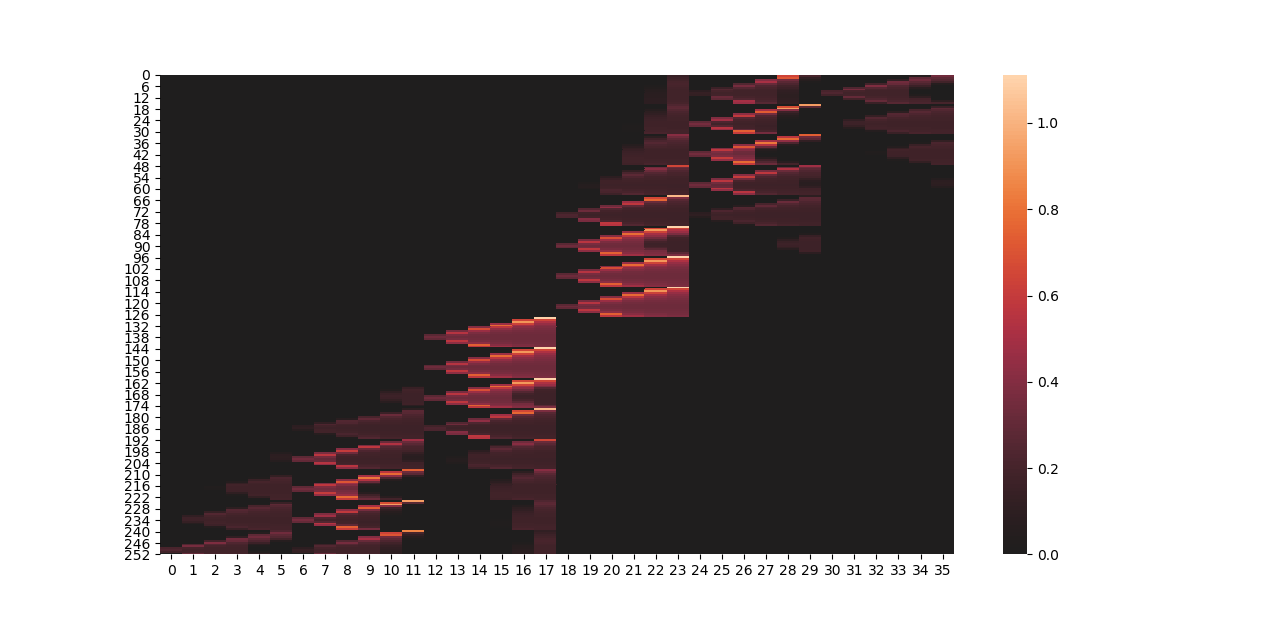
\includegraphics[width=14cm, height=10cm]{fig/matrix_1.png}
\end{figure}

Данная матрица является прямоугольной, поэтому выберем из неё квадратную неособенную матрицу. Выбирать будем по следующему принципу. Можео заметить, что данная матрица содержит 4 блока, 2 из которых нулевые. Рассмотрим ненулевой блок.

\begin{figure}[H]
    \centering
    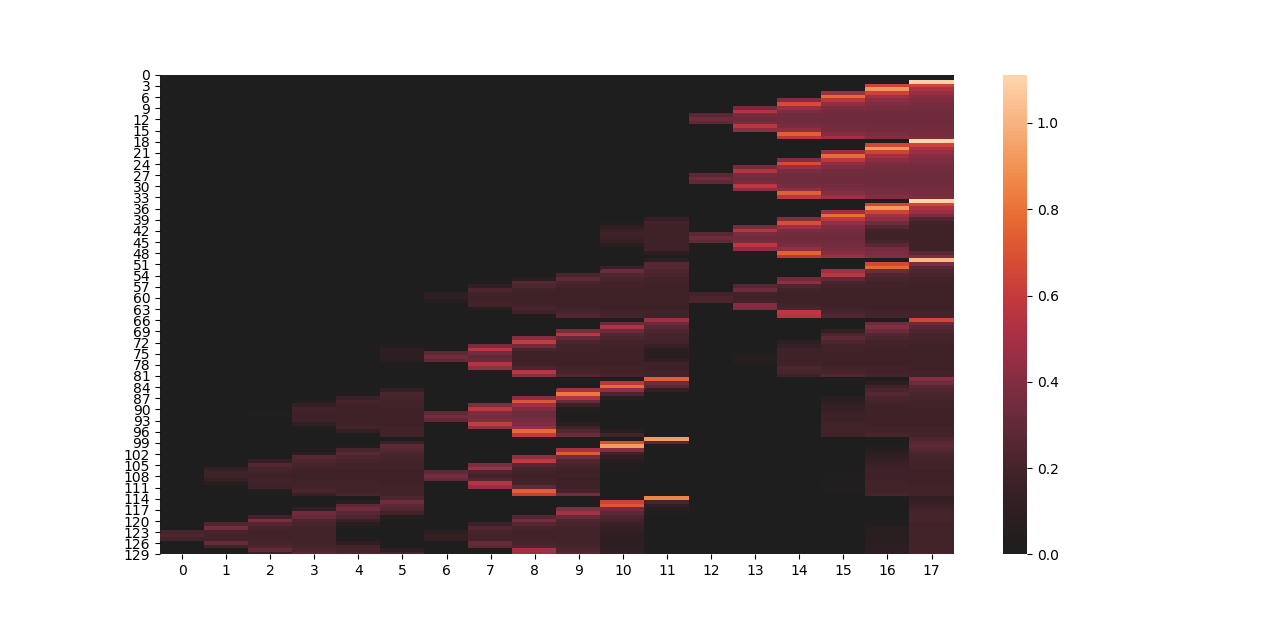
\includegraphics[width=14cm, height=10cm]{fig/matrix_1_nonzero.png}
\end{figure}

Здесь путём вырезания случайных строк из матрицы найдём неособенную квадратную матрицу. Получим следующую матрицу:

\begin{figure}[H]
    \centering
    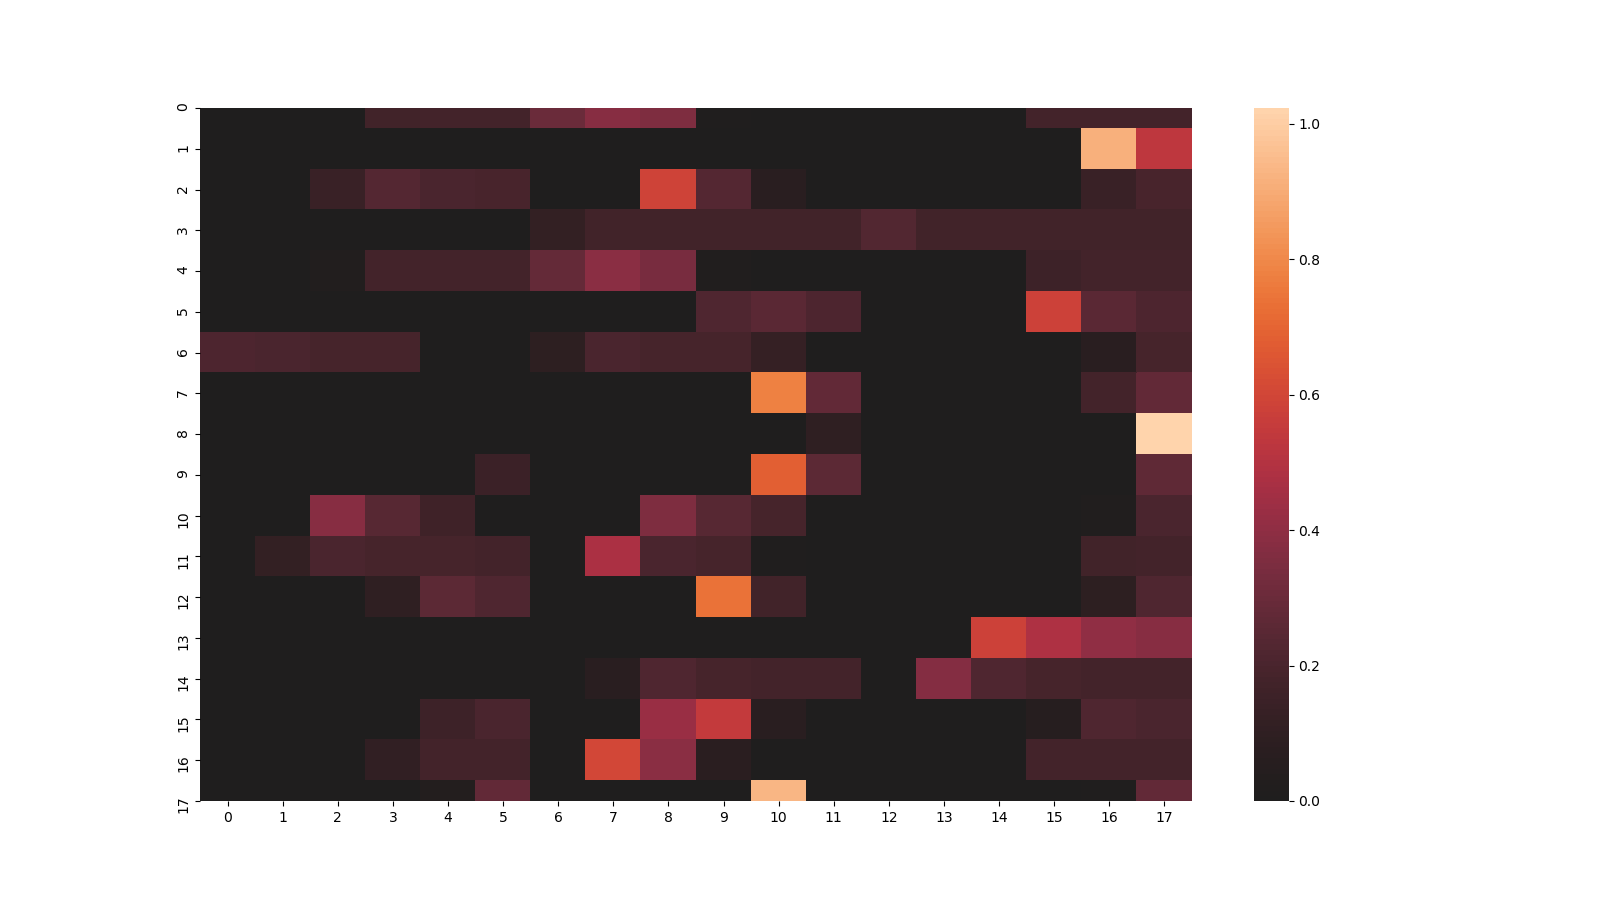
\includegraphics[width=14cm, height=10cm]{fig/nonspecial_1.png}
\end{figure}

Для танной матрицы сгенерируем случайный вектор $x$, а для него получим $b = Ax$, из него сгенерируем интервальный вектор $\bold b$. Решим задачу при помощи субградиентного метода Ньютона с заданной точностью $\varepsilon = 10^{-9}$. Представим полученные данные на графике.

\begin{figure}[H]
    \centering
    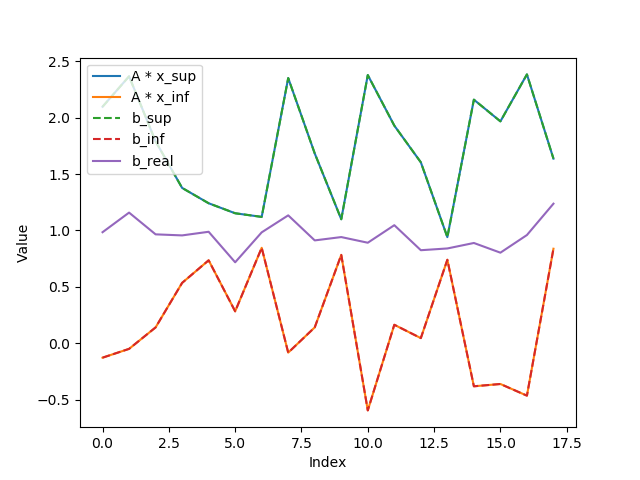
\includegraphics[width=14cm, height=10cm]{fig/b_comp_1.png}
	\caption{Сравнение правых частей}
\end{figure}

\begin{figure}[H]
    \centering
    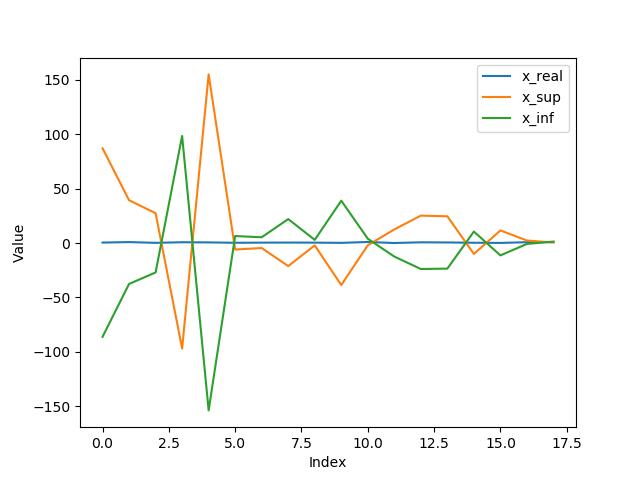
\includegraphics[width=14cm, height=10cm]{fig/x_comp_1.png}
	\caption{Сравнение решений}
\end{figure}

Из графиков видно, что оценка правой части достаточно хороша, реальные значения находятся в пределах интервала. Совершенно иначе дело обстоит с оценкой вектора $x$, здесь были получены неправильные интервалы, а оценка для некоторых элеиентов довольно груба, хотя реальное значение также содержится в пределах интервала

\subsubsection{2 вариант}

Имеем матрицу, которая схожа с матрицей из прошлого варианта тем, что в ней имеется 4 блока, из которых 2 нулевые. 

 \begin{figure}[H]
    \centering
    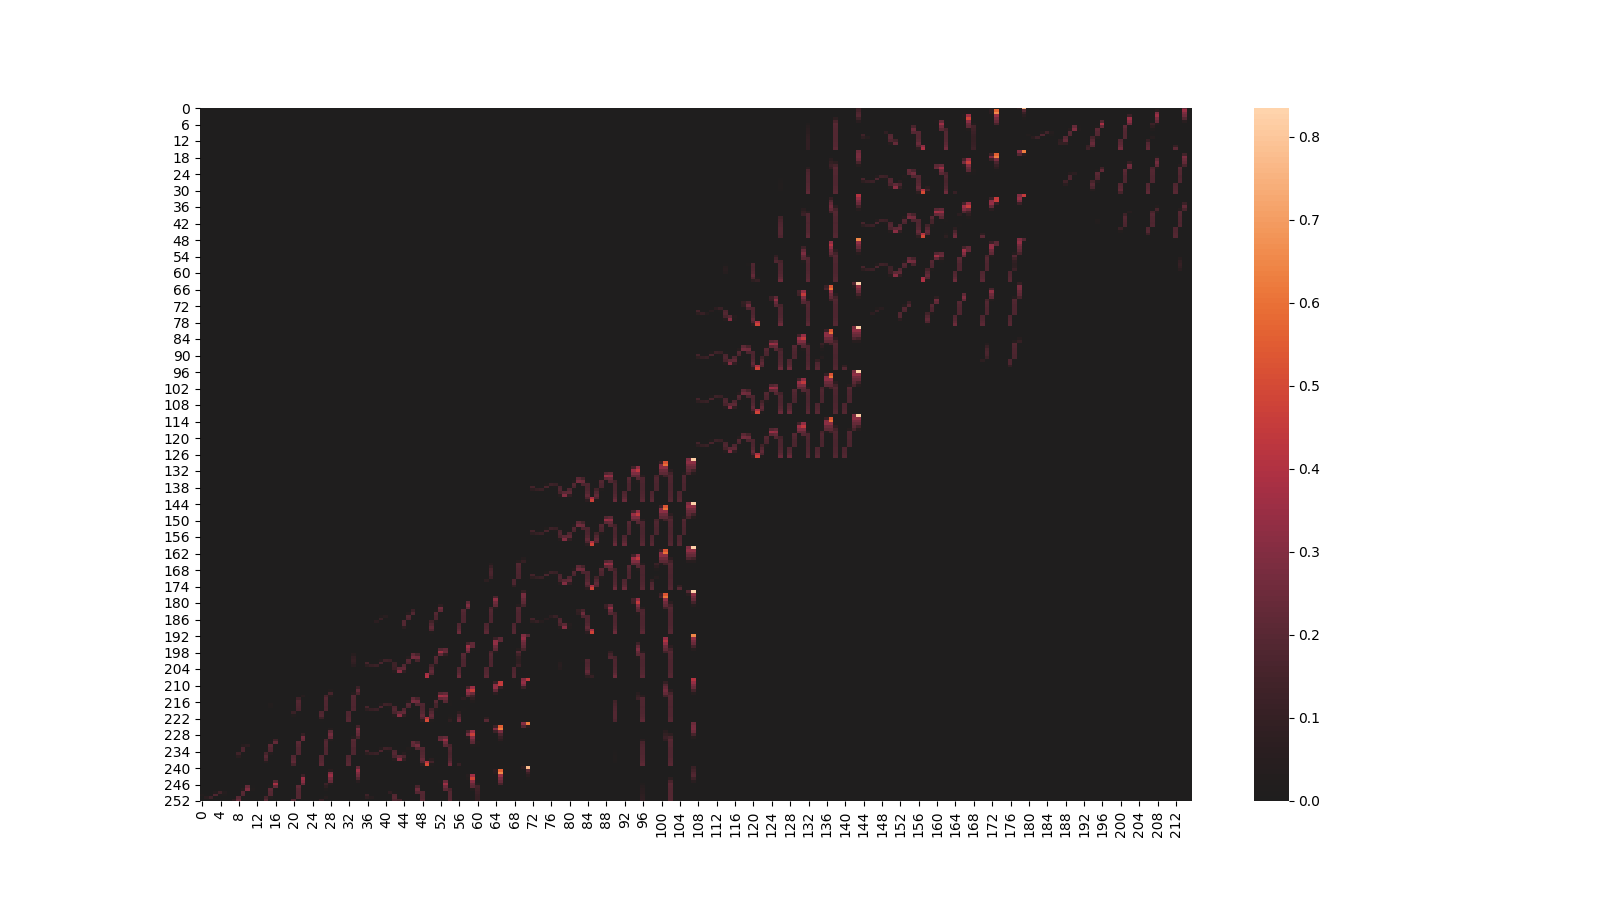
\includegraphics[width=14cm, height=10cm]{fig/matrix_2.png}
\end{figure}

Проведём аналогичные рассуждения.

\begin{figure}[H]
    \centering
    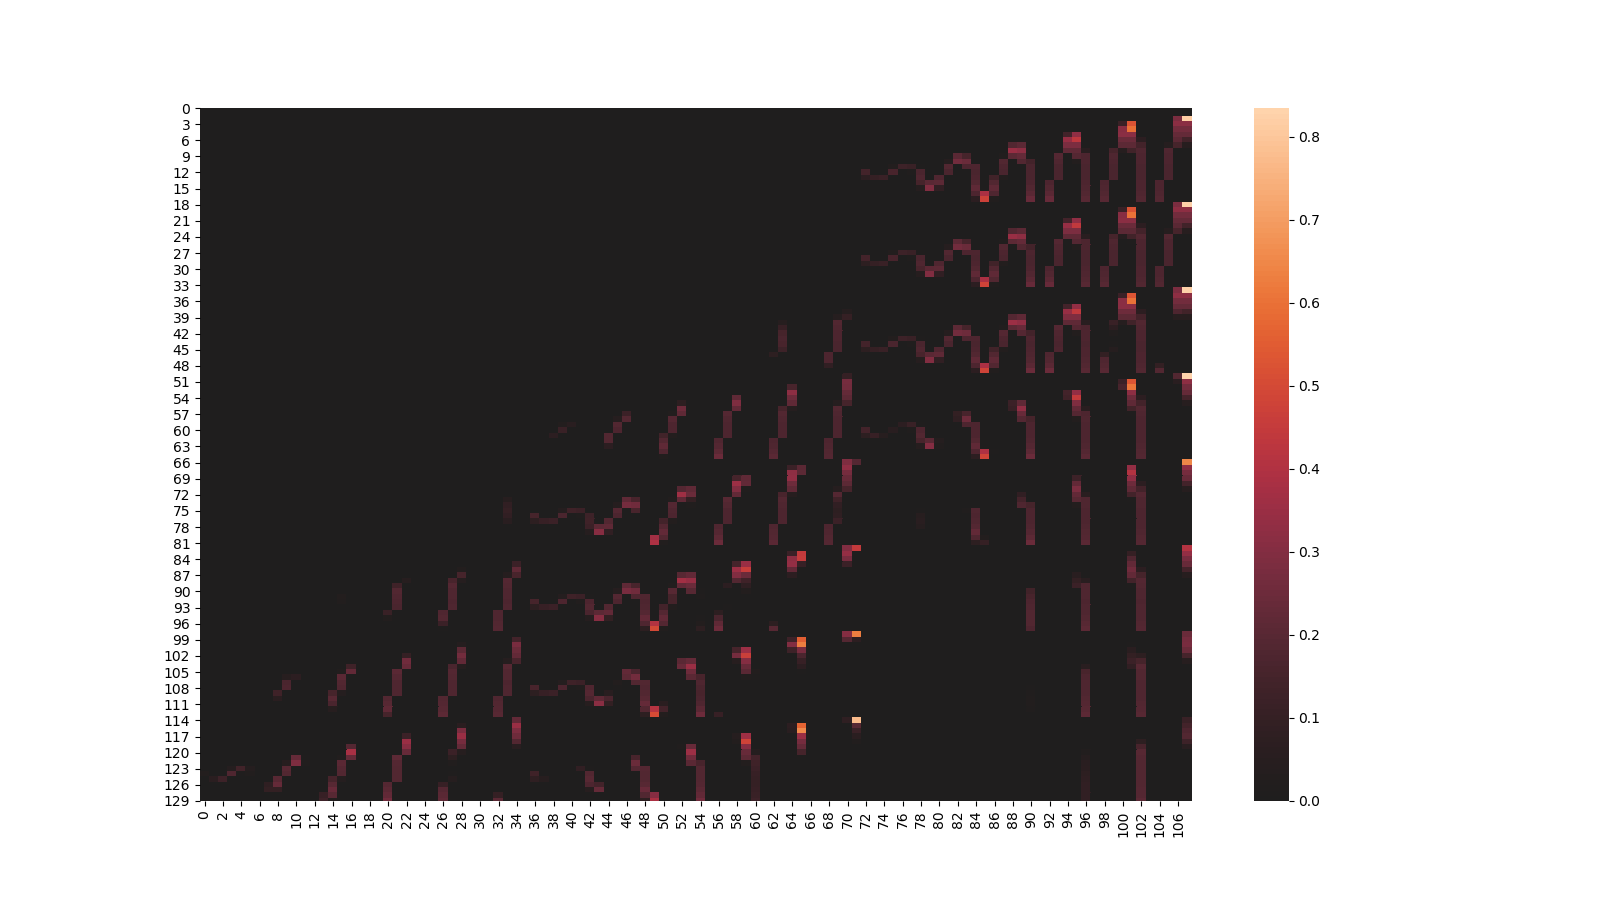
\includegraphics[width=14cm, height=10cm]{fig/nonzero_2.png}
	\caption{Ненулевая область}
\end{figure}

\begin{figure}[H]
    \centering
    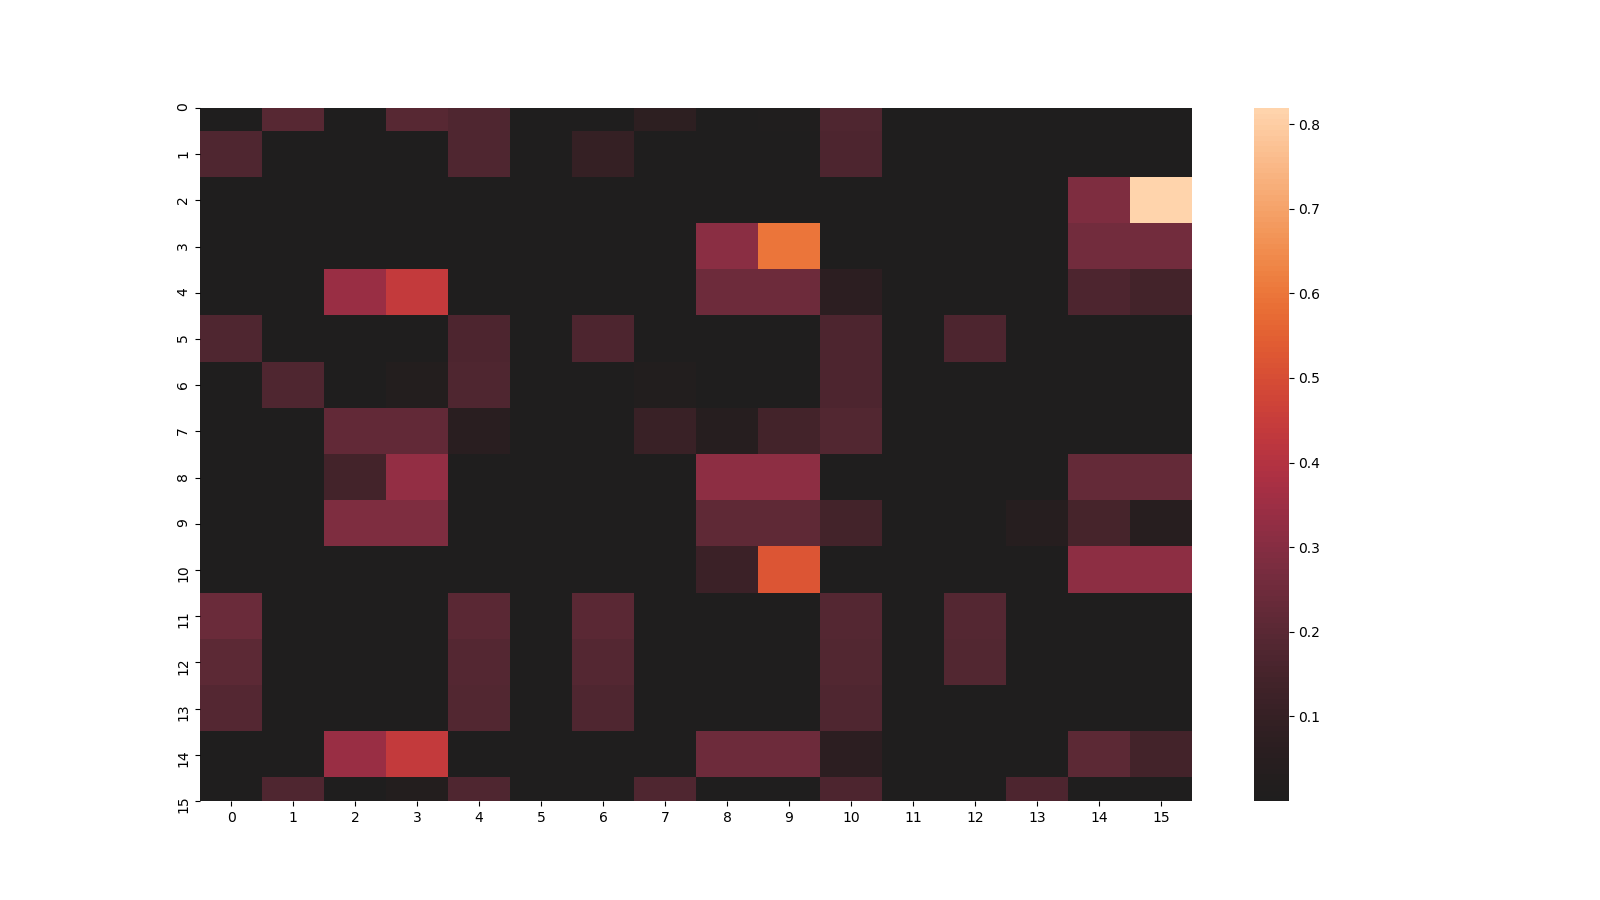
\includegraphics[width=14cm, height=10cm]{fig/nonspecial_2.png}
	\caption{Найденная неособенная область}
\end{figure}

 В этом случае имеем следующие результаты:

\begin{figure}[H]
    \centering
    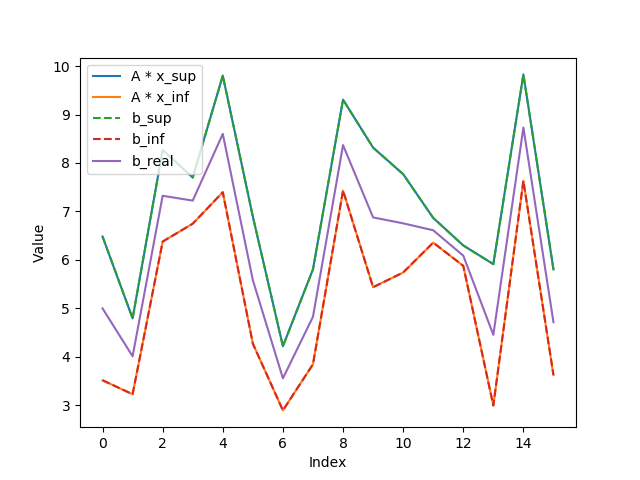
\includegraphics[width=14cm, height=10cm]{fig/b_comp_2.png}
	\caption{Сравнение правых частей}
\end{figure}

\begin{figure}[H]
    \centering
    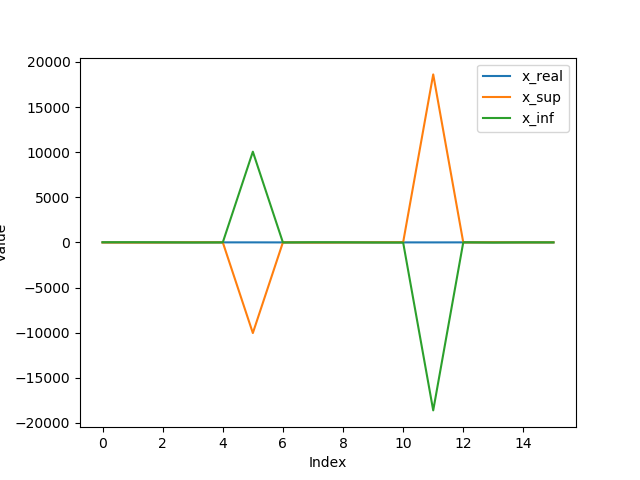
\includegraphics[width=14cm, height=10cm]{fig/x_comp_2.png}
	\caption{Сравнение решений}
\end{figure}

Результаты аналогичны прошлому варианту. Правая часть оценивается довольно хорошо. А для вектора решения наблюдаются те же проблемы: неправильные интервалы, грубая оценка.

\section {Реализация}
Лабораторная работа выполнена с помощью встроенных средств языка программирования Python.

\section{Приложения}
Репозиторий на GitHub с релизацией: \href{https://github.com/WiillyWonka/Intervals}{github.com}.
\end{document}
